%
% Main document
% ===========================================================================
% This is part of the document "Project documentation template".
% Authors: brd3, ngm1, hga3, sdl3
%



%---------------------------------------------------------------------------
% define document class
%---------------------------------------------------------------------------
\documentclass[
	 a4paper			% paper format
	,10pt				% fontsize
%	,twoside			% double-sided
%	,parskip=half			% set paragraph skip to half of a line
]{scrartcl}				% KOMA-script report
%---------------------------------------------------------------------------


%---------------------------------------------------------------------------
% Set up page dimension
%---------------------------------------------------------------------------
\usepackage[
	a4paper
	,left=30mm
	,right=15mm
	,top=25mm
	,headheight=0mm
	,headsep=10mm
	,footskip=15mm
]{geometry}
%---------------------------------------------------------------------------



%---------------------------------------------------------------------------
% Load Packages:
%---------------------------------------------------------------------------
\usepackage{template/sty/bfh}
% Packages:
%---------------------------------------------------------------------------
\usepackage{fancyhdr}					% simple manipulation of header and footer
\usepackage{pdflscape}					% allow switching to landscape
\usepackage{multicol}					% allows the creation of multicols
\usepackage{chngcntr}					% allows changing the context of counters
\usepackage{pdfpages}
\usepackage[standard-baselineskips]{cmbright}		% Computer Modern Bright fonts (a family of sans serif fonts)
\usepackage[utf8]{inputenc}				% load charset UTF8
\usepackage[T1]{fontenc}				% hyphenation of words with , and
\usepackage{ae}						% better resolution of Type1-Fonts
\usepackage{graphicx}					% integration of images
\usepackage{float}					% floating objects
\usepackage{caption}					% for captions of figures and tables
\usepackage{booktabs}					% package for nicer tables
\usepackage{tocvsec2}					% provides means of controlling the sectional numbering
\usepackage{lmodern}					% use modern font
\usepackage{titlesec}
\usepackage{wrapfig}
\usepackage[export]{adjustbox}
\usepackage{lastpage}
\usepackage[ngerman, num]{isodate}
\usepackage{amsmath}					% various features to facilitate writing math formulas
\usepackage{amsthm}					% enhanced version of latex's newtheorem
\usepackage{amsfonts}					% set of miscellaneous TeX fonts that augment the standard CM
\usepackage{amssymb}					% mathematical special characters
\usepackage{exscale}					% mathematical size corresponds to textsize
\usepackage{multirow}					% multirow emables combining rows in tables
\usepackage{tabularx}
\usepackage{tcolorbox}
\usepackage{csvsimple}
\usepackage{color}
\usepackage{listings}
\usepackage[acronym, toc]{glossaries}
\usepackage{lipsum}
\usepackage{makecell}
%---------------------------------------------------------------------------
% new bibliography using biber and biblatex
%    >> breaks cite package. Patch below provides
%    >> a patch to use cite
%---------------------------------------------------------------------------
\usepackage[
    backend=biber,
    style=ieee-alphabetic,
    sortlocale=de_DE,
    natbib=true,
    url=true,
    doi=true,
    eprint=false
]{biblatex}
\usepackage{xpatch}
\makeatletter
\xpatchcmd{\@citex}{\bfseries ?}{\bfseries\expandafter\strip@prefix\meaning\@citeb}{}{}
\makeatother
%---------------------------------------------------------------------------

\usepackage{template/sty/thesis}
\usepackage{lipsum}
%---------------------------------------------------------------------------


%---------------------------------------------------------------------------
% Define document properties
%---------------------------------------------------------------------------
\newcommand{\institution}{Berner Fachhochschule}
\newcommand{\fieldofstudies}{Informatik}
\newcommand{\course}{CAS CLD FS20~ -- Cloud Computing}

\newcommand{\doctype}{Semesterarbeit}
\newcommand{\doctitle}{Informatik}
\newcommand{\docsubject}{Geodatenprozessierung mit Budget Instanzen}

\newcommand{\docauthor}{Tobias Reber}

\newcommand{\prof}{Jörg Thomann}

\newcommand{\titleImage}{hippie_car}


%---------------------------------------------------------------------------


%---------------------------------------------------------------------------
% Hyperref Package (Create links in a pdf)
%---------------------------------------------------------------------------
\usepackage[
	pdftex
	,ngerman
	,bookmarks
	,plainpages=false
	,pdfpagelabels
	,backref = {false},		% No index backreference
	,colorlinks = {true},		% Color links in a PDF
	,hypertexnames = {true},	% no failures "same page(i)"
	,bookmarksopen = {true},	% opens the bar on the left side
	,bookmarksopenlevel = {0}	% depth of opened bookmarks
	,pdftitle = {\doctitle}		% PDF-property
	,pdfauthor = {\@author}		% PDF-property
	,pdfsubject = {\docsubject}	% PDF-property
	,linkcolor = {BFHlink}		% Color of Links
	,citecolor = {BFHlink}		% Color of Cite-Links
	,urlcolor = {BFHlink}		% Color of URLs
]{hyperref}
%---------------------------------------------------------------------------


%---------------------------------------------------------------------------
% usefull commands
%---------------------------------------------------------------------------
\def\matlab{{\em MatLab}}
\def\octave{{\em Octave}}
\newcommand{\includecode}[2][c]{\lstinputlisting[caption=#2, language=#1]{#2}}
\usepackage[nottoc,notlot,notlof]{tocbibind}
%---------------------------------------------------------------------------

% ---------------------------------------------------------------------------
% Bibliography resource
% --------------------------------------------------------------------------

\addbibresource{bibliography.bib}
%\bibliography{bibliography}
%\bibliographystyle{abbrv}


% ---------------------------------------------------------------------------
% Graphic paths
%---------------------------------------------------------------------------
\graphicspath{{template/}{pictures/}{svg/}}

%---------------------------------------------------------------------------
% The document
%---------------------------------------------------------------------------
\begin{document}
% Title
%---------------------------------------------------------------------------
\pagestyle{empty}
\thispagestyle{empty}

%% include BFH logo and HuCE-ml logo
\begin{figure}
	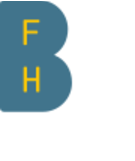
\includegraphics[scale=1,valign=t]{BFH_Logo_A_en_100_4CU.pdf}
\end{figure}

%% Document title and subtitle

\begin{minipage}[c][3cm][c]{\linewidth} {
	\centering
	\vspace*{2cm}
	{\fontsize{24pt}{0pt}\selectfont \textbf{\doctitle}}  \\
	\vspace*{0.6cm}
	{\fontsize{20pt}{0pt}\selectfont {Geodeatenprozessierung\\ mit Budget Instanzen}}  \\
	\vspace*{1cm}
	{\fontsize{14pt}{0pt}\selectfont \doctype}  \\
}
\end{minipage}


\vspace{1.5cm}


%% Title image
\begin{figure}[H]
	\centering
	\makebox[0.8\linewidth]{\color{BFHGray} \rule{0.8\linewidth}{10pt}}
	\includegraphics[width=.8\textwidth,height=9cm,keepaspectratio]{\titleImage}
	\makebox[0.8\linewidth]{\color{BFHGray} \rule{0.8\linewidth}{10pt}}
    \caption{Eine Ausfahrt mit Budget Instanzen\space\cite{HippieCar:1}}
\end{figure}

\vfill

%% Author and document information
\begin{minipage}[c][3cm][c]{\linewidth}
{
	\centering
	\begin{tabbing}
		xxxxxxxxxxxxxxxxxxx\=xxxxxxxxxxxxxxxxxxxxxxxxxxxxxxxxxxxxxxxxxxxxxxx \kill
		Departement:	\> \fieldofstudies \\
		Kurs:			\> \course \\
		Autor:		\> \docauthor \\
		Experte:		\> \prof \\
		Datum:			\> \today \\
	\end{tabbing}
}
\end{minipage}

\pagebreak

%---------------------------------------------------------------------------
% Lead
%---------------------------------------------------------------------------
\startLead
%########################################################################################################
%THE INTRO WITH Kahlil Gibran
%########################################################################################################


\newpage \vspace*{8cm}
\label{har:perplexity}
\begin{center}
\large Perplexity\\
is the beginning of knowledge.
\vspace{4mm}
\\
- Kahlil Gibran\\
\vspace{2mm}
\autocite[33]{CloudNativ:1}
\end{center}


\newpage
\section*{Management Summary}
In der Kürze liegt die Würze \autocite{DUMMY:1}

\pagebreak
\setlength{\parskip}{0pt}

%% Tabel of contents
\makeatletter
\renewcommand{\tableofcontents}{%
	\vspace*{0em}% reduce space before
	\noindent{\Large\contentsname\par}%
	\vspace{2mm}% space between title and rule
	\hrule
	\vspace{2mm}% space below rule
	\@starttoc{toc}
	\vspace{4mm}
	\hrule
}

\makeatother
\renewcommand{\contentsname}{Inhaltsverzeichnis}
\setcounter{tocdepth}{3}

\tableofcontents\label{toc}
\setlength{\parskip}{10pt}

\pagebreak

\setlength{\parskip}{0pt}

\makeatletter
\renewcommand{\listoffigures}{%
	\vspace*{0em}% reduce space before
	\noindent{\Large\listfigurename\par}%
	\vspace{2mm}% space between title and rule
	\hrule
	\vspace{2mm}% space below rule
	\@starttoc{lof}
	\vspace{4mm}
	\hrule
}

\makeatother
\renewcommand{\listfigurename}{Abbildungsverzeichnis}

\listoffigures\label{lof}
\setlength{\parskip}{10pt}

\pagebreak
%---------------------------------------------------------------------------
% Contents
%---------------------------------------------------------------------------
\startMainPart
\section{Samples}
This is an example document 
\lipsum[1-3]

\clearpage
\section{Images}
\begin{figure}[H]
	\centering
	
\includegraphics[width=.6\textwidth]{placeholder}
	\caption{Overview of the frames used}
	\label{fig:placeholder}
\end{figure}

\begin{multicols}{2}
	\begin{figure}[H]
		\centering
		
\includegraphics[width=.45\textwidth,angle=90]{placeholder}
		\caption{PCB design in 3D (top view)}
		\label{fig:multicol:placeholder1}
	\end{figure}

	\begin{figure}[H]
		\centering
		
\includegraphics[width=.45\textwidth]{placeholder}
		\caption{PCB design in 3D (bottom view)}
		\label{fig:multicol:placeholder2}
	\end{figure}
\end{multicols}


\section{Table}
\begin{center}
	\begin{tabular}{ | l | l | l | p{5cm} |}
		\hline
		Day & Min Temp & Max Temp & Summary \\ \hline
		Monday & 11C & 22C & A clear day with lots of sunshine.  
		However, the strong breeze will bring down the temperatures. \\ \hline
		Tuesday & 9C & 19C & Cloudy with rain, across many northern regions. Clear spells 
		across most of Scotland and Northern Ireland, 
		but rain reaching the far northwest. \\ \hline
		Wednesday & 10C & 21C & Rain will still linger for the morning. 
		Conditions will improve by early afternoon and continue 
		throughout the evening. \\
		\hline
	\end{tabular}
\end{center}

%\begin{center}
%	\begin{tabular}{l|c}%
%		\bfseries Person & \bfseries Matr.~No.% specify table head
%		\csvreader[head to column names]{grade.csv}{}% use head of csv as column names
%		{\\\hline\givenname\ \name & \matriculation}% specify your coloumns here
%	\end{tabular}
%\end{center}

\subsection{Testing}
Dies ist der Unterttitel

\section{Lists}
\begin{itemize}
	\item sample list item
\end{itemize}

\begin{enumerate}
	\item sample list item
\end{enumerate}

\section{Code}
\begin{lstlisting}
touch --help
nano --help
mkdir --help
\end{lstlisting}

\lstinputlisting[language=C,caption=Sample C Code]{src/sampleCode.c}


\section{Equations}
This is an equation: $F = m \cdot a$

Here are some more:
\begin{align}
	y &= mx + b \\
	c^2 &= a^2 + b^2
\end{align}

and even more:
\begin{align*}
	y &= mx + b \\
	c^2 &= a^2 + b^2
\end{align*}




%---------------------------------------------------------------------------
% Bibliography
%---------------------------------------------------------------------------
\cleardoublepage
\phantomsection
\addcontentsline{toc}{section}{Literaturverzeichnis}
\renewcommand{\bibname}{Literaturverzeichnis}
\printbibliography


%---------------------------------------------------------------------------
% Appendix
%---------------------------------------------------------------------------
\startAppendix
\section{Demo Anhang}\label{app:demo}
\appendCode{c}{Sample Code}{src/sampleCode.c}


%---------------------------------------------------------------------------
\end{document}
%---------------------------------------------------------------------------

